\section{Tecnolog\'ia a Utilizar}
\label{sec:tecnologia-utilizada}

Como expone la secci\'on~\ref{sec:problema-especifico}, se decidi\'o dise\~nar
una interfaz para componer m\'usica utilizando la voz. Adem\'as, desde un principio
este trabajo de grado opt\'o por la metodolog\'ia de trabajo
de C\'odigo Abierto, lo cual implica: 

\begin{itemize}
    \item Utilizar tecnolog\'ias de C\'odigo abierto para el desarrollo de la interfaz.
    \item Establecer un proceso de desarrollo transparente y abierto.
    \item Ofrecer la interfaz desarrollada, junto con su código fuente, de manera libre 
        y gratuita para la comunidad de Código Abierto.
\end{itemize}

La metodolog\'ia adoptada para implementar la interfaz permiti\'o utilizar un proyecto
existente como punto de partida, y as\'i a\~nadir soporte para comandos de voz. Adem\'as,
el hecho de incorporar una nueva interfaz, permite analizar
una de las motivaciones de la secci\'on~\ref{sec:motivacion}: un programa de composici\'on
musical, que recibe comandos sonoros y emite tambi\'en un resultado sonoro, podr\'ia ser
m\'as natural para el usuario. A continuaci\'on se presenta el proyecto de C\'odigo Abierto
utilizado como punto de partida para la soluci\'on implementada.

\subsection{TamTam Edit}

La m\'usica es a menudo descrita como la forma m\'as pura de representaci\'on matem\'atica, es m\'as, te\'oricos de la
m\'usica han utilizado las matem\'aticas para resolver problemas musicales \cite{TheSoundOfNumbers}. Esto sirvi\'o
de inspiraci\'on para la creaci\'on del compendio de actividades\footnote{Una Actividad, es una aplicaci\'on en el entorno 
de escritorio \emph{Sugar}}
conocido como \emph{TamTam} desarrollado para la computadora XO\footnote{La XO, es una computadora 
port\'atil de bajo costo y consumo desarrollada por el proyecto \emph{One Laptop Per Child}},
con los siguientes objetivos:

\begin{itemize}
    \item Proveer a los niños un ambiente de información cultural construyendo música y sonidos.
    \item Brindar una experiencia sonora/musical divertida para usuarios sin conocimientos musicales.
    \item Promover un camino hacia experiencias musicales más sofisticadas.
    \item Promover un instrumento musical con su propio ``sonido''.
    \item Desarrollar un ambiente dinámico y mutable que propone la simpleza y permite la complejidad.
    \item Favorecer la creación de música grupalmente.
    \item Introducir los conceptos musicales y otros como: programación y audio.
\end{itemize}

\emph{TamTam Edit} es una aplicaci\'on, que forma parte del conjunto de actividades musicales \emph{TamTam}, que proporciona
una interfaz intuitiva para crear, modificar y organizar notas ubicadas en pistas virtuales. Adem\'as incluye una paleta de
casi cien tipos de sonidos y modelos de construcci\'on musical que permite crear distintos tipos de variaciones en estilos
musicales \cite{TamTamWiki}.


Las secciones principales del programa se pueden observar en la figura~\ref{figure:ui-tamtam} 

\begin{figure}[H]
\centering
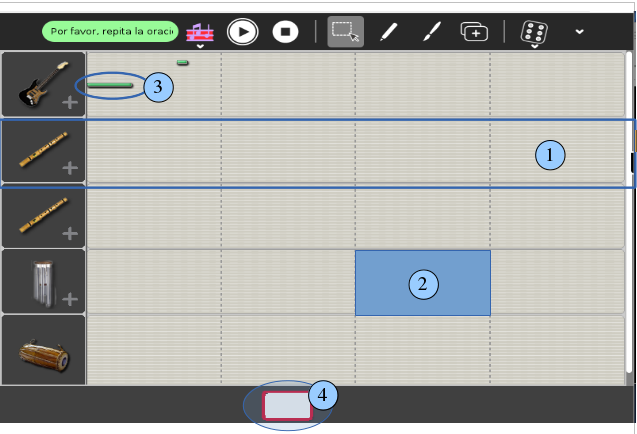
\includegraphics[width=\textwidth]{./graphics/ui-tamtam-edit.png}
\caption{Interfaz de \emph{Tamtam Edit} y sus secciones principales}
\label{figure:ui-tamtam}
\end{figure}

Como se puede apreciar en la figura~\ref{figure:ui-tamtam}, la interfaz se encuentra organizada en cinco pistas y cada pista tiene asociada un 
instrumento (la quinta pista esta reservada para instrumento de tipo batería). Cada pista se divide en 4 
compases (del compás uno al cuatro) y cada compás se divide en 12 tiempos (del uno al doce). 
Las notas se dibujan en los compases, como se puede ver, la longitud de la nota indica su duración y su 
altura el tipo de nota. Además la aplicación esta organizada en partituras, que son como hojas de 
cuaderno, y son útiles para componer músicas largas.

La interfaz de la figura~\ref{figure:ui-tamtam} ofrece una experiencia de interacci\'on humano-computadora tradicional. 
Este trabajo de grado busca incorporar un medio de interacci\'on alternativo al propuesto por \emph{TamTam Edit}. 
A continuaci\'on se presentan los motivos que determinaron la elecci\'on de esta aplicaci\'on como punto de partida:

\begin{itemize}
    \item \emph{Impacto social:} \emph{TamTam Edit} es una aplicaci\'on que forma parte de una plataforma establecida
    por el proyecto \gls{olpc}. Este proyecto busca proveer
	a cada ni\~no de pa\'ises en desarrollo de una computadora de bajo costo con el
	fin de potenciar el proceso educativo \cite{OLPC}. Ni\~nos con alg\'un tipo de discapacidad podr\'ian tener
	problemas para utilizar la computadora. Por ejemplo, un ni\~no con problemas motrices podr\'ia tener dificultades para operar el mouse
	o el teclado. Para estos casos, operar esta actividad utilizando la voz beneficiar\'ia a los ni\~nos con discapacidades
	y por lo tanto la aplicaci\'on tendr\'ia un impacto social positivo, debido a la mejora en la accesibilidad.
    \item \emph{Naturalidad de interacci\'on:} utilizar la voz para interactuar con una aplicaci\'on presenta una mayor
	naturalidad con respecto al enfoque tradicional de interacci\'on, debido a que es el medio de
	interacci\'on entre las personas.
    \item \emph{No reinventar la rueda:} como el objetivo es incorporar una interfaz basada en reconocimiento del habla a una aplicaci\'on,
	se elige \emph{TamTam Edit} para no construir la aplicaci\'on desde cero, sino extender las capacidades de una ya existente.
    \item \emph{C\'odigo abierto:} el motivo anterior es posible gracias a que \emph{TamTam Edit} es un proyecto de c\'odigo abierto, lo cual
	brinda a los desarrolladores la libertad de extender las funcionalidades de la aplicaci\'on.
    \item \emph{Lenguaje de programaci\'on:} la actividad se encuentra implementada en el lenguaje de programaci\'on Python. Este es el
	lenguaje elegido para realizar la interfaz, adem\'as la librer'ia de reconocimiento del habla a ser utilizada proporciona
        \emph{bindings} para este lenguaje.
\end{itemize}



\subsection{PocketSphinx}

El cap\'itulo~\ref{sec:tecnologias} clasifica a las herramientas que permiten implementar soluciones
basadas en reconocimiento del habla en tres categor\'ias: Aplicaciones, \gls{api}s y Librer\'ias. Dada la naturaleza de \'este trabajo, se
ha optado por elegir una librer\'ia para implementar la interfaz alternativa a la ofrecida por
\emph{TamTam Edit}.

Para la implementaci\'on de la interfaz operable a trav\'es de la voz se ha elegido la librer\'ia \emph{PocketSphinx} que,
como se menciona en la secci\'on~\ref{sec:pocketsphinx}, es un motor de reconocimiento del habla orientado a la optimaci\'on
del rendimiento y la portabilidad.

Uno de los objetivos espec\'ificos de este trabajo de grado es aplicar y contrastar en la pr\'actica
los conocimientos te\'oricos adquiridos. Como indica la secci\'on~\ref{sec:librerias}, una librer\'ia es
el tipo de herramienta que requiere un conocimiento t\'ecnico espec\'ifico del \'area, adem\'as de
brindar una alta flexibilidad permitiendo al programador manipular los distintos componentes del
proceso de reconocimiento del habla. Por lo tanto una librer\'ia es la herramienta m\'as adecuada
para cumplir el objetivo mencionado anteriormente.

A continuaci\'on se presentan los motivos t\'ecnicos que determinaron la elecci\'on de esta librer\'ia:

\begin{itemize}
    \item Existen \foreign{bindings} para el lenguaje de programaci\'on Python, lo cual hace muy sencilla la tarea de utilizar
	la librer\'ia desde el c\'odigo Python.
    \item \emph{PocketSphinx} esta orientada a la optimizaci\'on del rendimiento, resultando adecuada para sistemas con
	recursos limitados, como es el caso de la computadora \emph{XO}.
    \item La librer\'ia es un proyecto de c\'odigo abierto, por lo tanto se cumple la metodolog\'ia de trabajo adoptada.
\end{itemize}
